\documentclass{article}
\usepackage[utf8]{inputenc}

\title{\LARGE WEATHER STATION}
\author{\LARGES S.Felipe \ 2420142004 ,{ L Kelly \ 2420151034} , S.D Luis\ 2420162033}
\date{University of  Ibague}
\usepackage{multicol}
\usepackage{hyperref}
\usepackage[hidelinks]{hyperref}
\usepackage{graphicx}
\begin{document}

\maketitle
\begin{multicols} {2}
\textbf{abstract}: 
This article presents the implementation of a weather station that allows to observe at the measurement site and remotely, the change of the different climatic variables such as: rain, temperature and relative humidity of the environment, atmospheric pressure, air quality. Initially, the respective characterization of the sensors used is, in fact, carried out by the specifications given by the manufacturer. After the characterization process, through the Arduino IDE Software the acquisition of the sensor data is made: raindrops and air quality MQ135, because these analog inputs, which are sent by serial communication between the arduino nano and the Raspberry pi 3b +, make conversion to digital signals. For the remaining DHT11, BMP180 and GPS sensors, perform the acquisition using a working code in python3, to finally acquire all the digital signals in a source code that allows the use of Wi-Fi from rasberry pi 3b +, they are uploaded to the platform Thingspeak web and additionally are saved in a .txt file that is sent by mail to the user every 12 hours, which have the specific information of the behavior of the variables and the location in real time where said measurement of their culture is made.
\\

\textbf{Keywords}: 
\textit{Arduino, weather station, raspberry pi 3b +, MQ135 sensor, BMP180 sensor, DHT11 sensor, GPS-NEO6M module, rain sensor, presipitation, temperature, air quality, atmospheric pressure, wet.}
\documentclass[9pt]{book}
\begin{center}
\section{INTRODUCTION}
\end{center}
Many farmers in the region are unaware of the real-time behavior of climate variables, which can affect their productive activities such as crop planning and planting. Therefore, the need arises to create a weather station that allows through the use of the internet of things, to have fast, reliable, and easy access to a web platform, which will be responsible for expressing the reading of these variables through graphics. With this, the farmer has a general management of all behaviors to take into account for the proper functioning of his crop in one part (THINGSPEAK). At the same time, thinking about it, he sent an email programmed every 12 hours, containing a txt file, with the behavior of each of the variables during that established time, adding the IP address where said station is being controlled and its location using a GPS module Dr. Rafael Belloso (2016, January 1). This so that the farmer can generate a solid database for possible weather predictions and a constant knowledge of how to plan their duties and functions for the crop.

At present, the market for meteorological stations has grown exponentially because every time the human being adapts to the development of innovation and technology Tobojas G. (2016). At the same time, they manage a wide market according to the needs of each client, due to the variety of stations that exist (pluviographic station, main weather station, ordinary weather station, main synoptic station, supplementary synoptic station, agrometeorological station). Even so, its sales costs are high, considering that not all customers have an economy for this type of product, which sometimes according to the manufacturer varies its functionality having more functions than other Morkerker, L (2019).

Our line of choice was evaluated taking into account the need of the region and the potential for selling the product, since we are located in a region that has high trade in agricultural products, such as cotton, rice, cocoa, coffee, reaching the conclusion that for agriculture turns out to be a device that can help you exponentially in your functions for the Smartic Research Seedbed crop. (2015).
 
Our purpose is to provide a service that meets the needs of the farmer, with the use of new technologies that allow multiple communication channels, detecting meteorological behaviors such as microclimates through precipitation sensors that open a line of research so that in the future they can develop preventive alarm systems in order to predict disasters Rojas, F. (2017).

\begin{center}
\section{OBJECTIVES}
\end{center}
\subsection{Overall Objective:}
\\
• Develop a real-time monitoring system for online monitoring of information that allows good planning in crop production activities.
\subsection{Specific objectives:}
• Design and implement the system hardware for the collection of variables: temperature, humidity, atmospheric pressure, air quality and precipitation.

• Develop an algorithm that manages the data obtained, processes it and makes publications and reports via the internet.

• Periodically publish the data collected in graphics through web platforms.

• Warn by means of an alert via email, about unexpected changes in the weather conditions established by the user.

\begin{center}
\section{THEORETICAL FRAMEWORK}
\end{center}
\subsection{Weather Station}
A weather station consists of a structure or device equipped with sensors
(temperature, humidity, atmospheric pressure, air quality, precipitation etc) that responds
to electrical stimuli, which allow to record and collect meteorological information in
automatically and in real time. This allows monitoring of variations of the
air temperature, relative humidity, atmospheric pressure, air quality, precipitation [6].

\subsection{environmental variables}
When installing a weather station, the sensors and
that way to make measurements of some environmental variables which are:

\textbf{Air temperature}: Temperature is the measure of the heat content of a body
or of the environment. In the vast majority of stations, it is measured in degrees Celsius (° C).
By measuring this, the influence of temperature on the speed at which the crops develop can be measured. [5]

\textbf{Rainfall}: Precipitation is the direct fall of water droplets or ice crystals on the earth's surface. The measurement is performed by means of a rain gauge and units in millimeters (mm) are generally used [6].

\textbf{humidity}: Ambient humidity is the measure that tells us the amount of water vapor present in the air. It is represented in percentage or degree of humidity[5].

\subsection{Weather stations classification}
Weather stations can be classified according to the application they are going to Directed its development.

* \textbf{Agro meteorological}: Focused on the observation study
biological and its relationship between climatic factors and the cycle of beings Live in this. Relations between time, weather, plant, animals, etc[4].

*\textbf{Climatological}:Focused on the study through systems of
sensors related phenomena such as: atmospheric time, quantity,
visibility, rainfall, air temperature, humidity[2].


\begin{center}
\section{RESULTS} 
\end{center}
\subsection{Description of the Weather Station.}

With the objective of solving our approach to the problem, we began to analyze what kind of variables were important to work in order to choose a weather station line to be carried out, choosing the main weather station which is that weather station that is provided to make observations of the current weather, quantity, visibility, precipitation, air temperature, humidity, and other special phenomena. Which normally performs about three daily measurements, but in order for the client to have more detailed information, we decide to send the data in real time, dividing the data every 12 Hours, adding to them the location of said station and the IP that it controls it and allows the sending of data via Wi-Fi to the web platform and to the determined email.

As we can see in Figure 1. Block diagram, with their respective inputs and outputs, and interconnection thereof, we chose 5 sensors that would be responsible for obtaining data (DTH11, DUAL MAQ-135, BMP180, RAIN SENSOR, GPS-NEO), we developed the codes of the sensors (BMP180, GPS-NEO, DTH11) directly from python3 since they have digital input, and for the sensor MAQ-135 DUAL and RAIN SENSOR we use an Arduino due to its analog inputs, then we generate a base code, which it would allow us to run all the code in Python 3, simultaneously, interlacing each of the functions. Having all the part of the Software, we are concerned with the design of the hardware, taking into account that said station must be outdoors and may be subject to rain or sudden climatic changes, we decide how it can be seen in Image 1 Mete Station rheological, it was necessary to use two electrical boxes interconnected by a LAN cable, one in which all those components that should not enter the water such as RAS, BATTERY, GPS could be placed.

And another one in which those sensors were needed that needed air or rain for its correct reading, opening holes in established points that do not affect the operation of any of the sensors. In this way we reach the final product.

\subsection{Development and Procedures of
Characterization}

Initially, the data obtained from the aforementioned variables will be displayed on the location site of the weather station, then take them remotely by using the internet of things to a web platform like Thingspeak, in turn saving them in a file .txt that will be called by a function every 12 hours to later send them via email next to the IP address from where the system is controlled, and a link that redirects directly to Google Maps showing the location in real time. Figure [1] shows the procedure diagram used.


\begin{center}
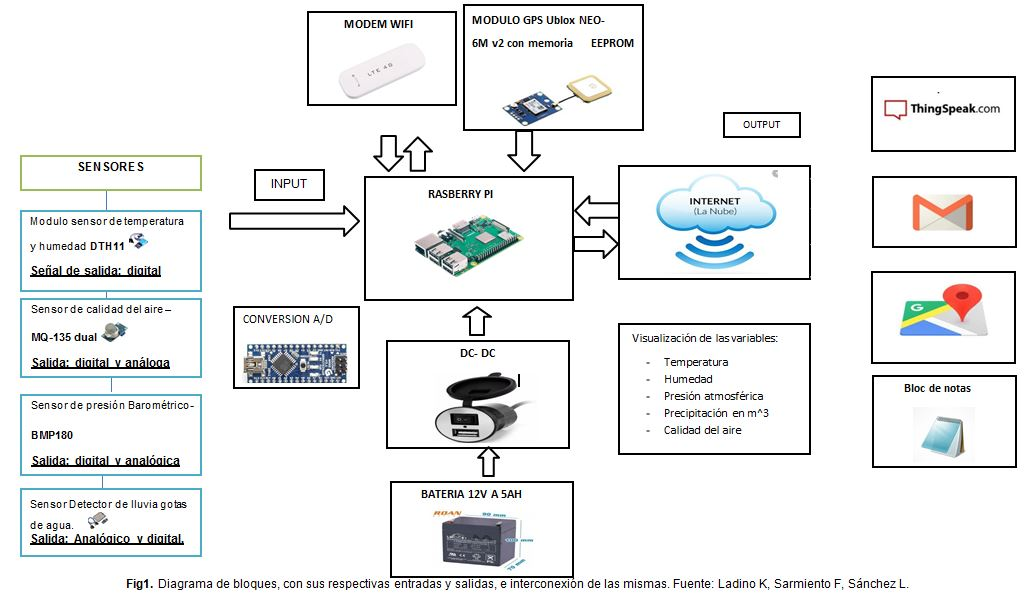
\includegraphics[scale=0.2]{Captura.JPG}
\caption{Figure [1] System inputs and outputs}
\end{center}

\textbf{characterization of the sensors in arduino}:

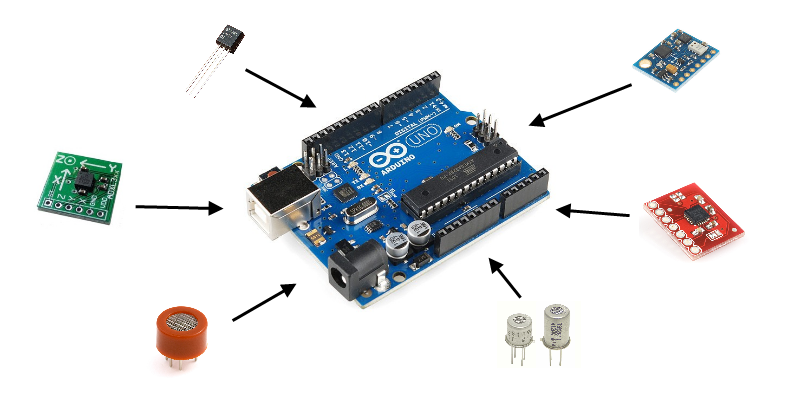
\includegraphics[scale=0.2]{arduino.png}

\caption{Fig{2}: Sensors in Arduino.}
\\\\

\textbf{
visualization of the behavior of the sensors graphically in real time}:

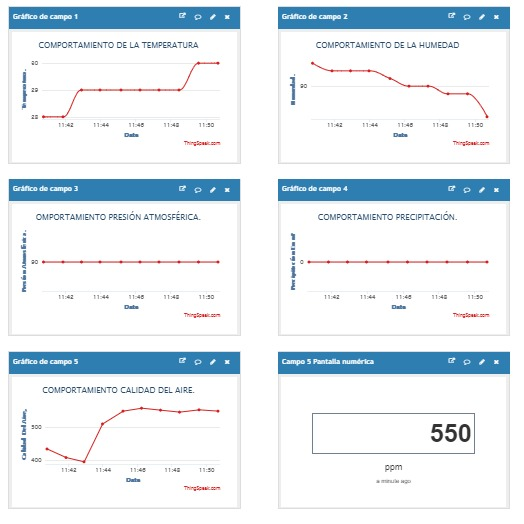
\includegraphics[scale=0.28]{grafico.jpg}

\caption{Fig[3] Checking Variables in Time}
\\

\textbf{Acquisition of data saved in a .txt file}:
\begin{center}
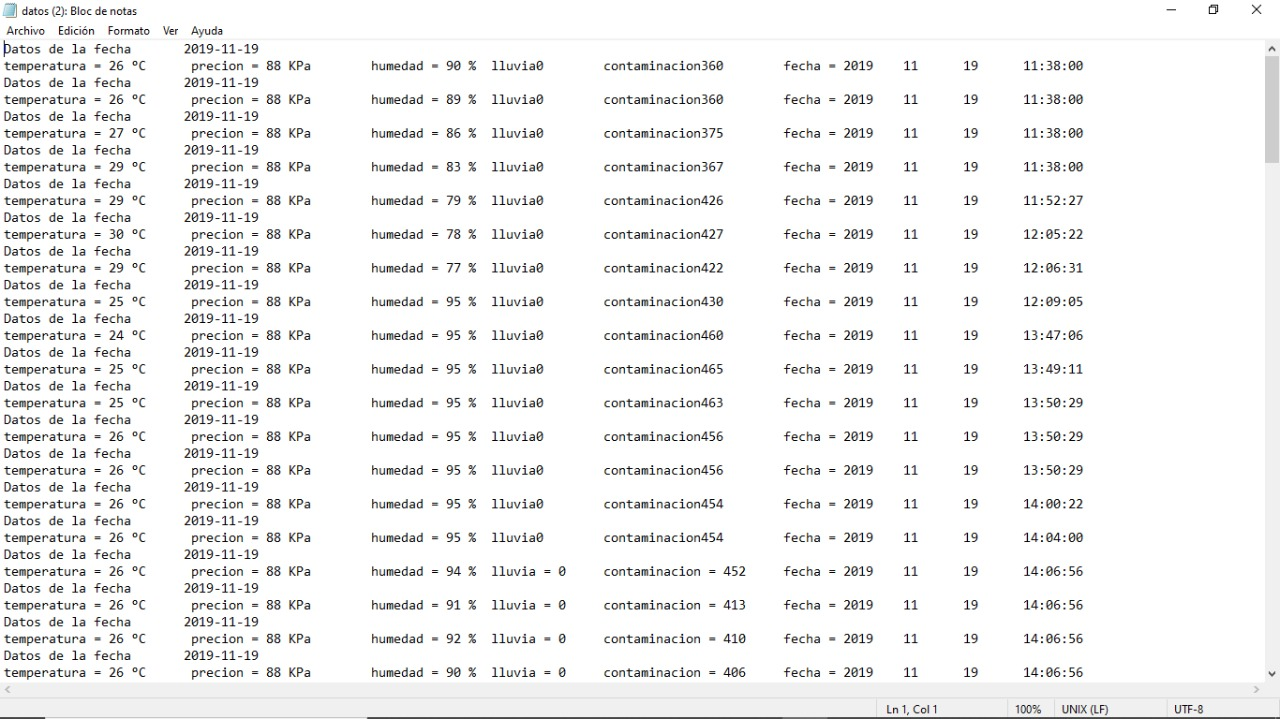
\includegraphics[width=0.4\textwidth]{diagrama.jpeg}
\\
\caption{Fig[4] Archivo .txt}
\end{center}

\textbf{E-mail sent}:

\begin{center}
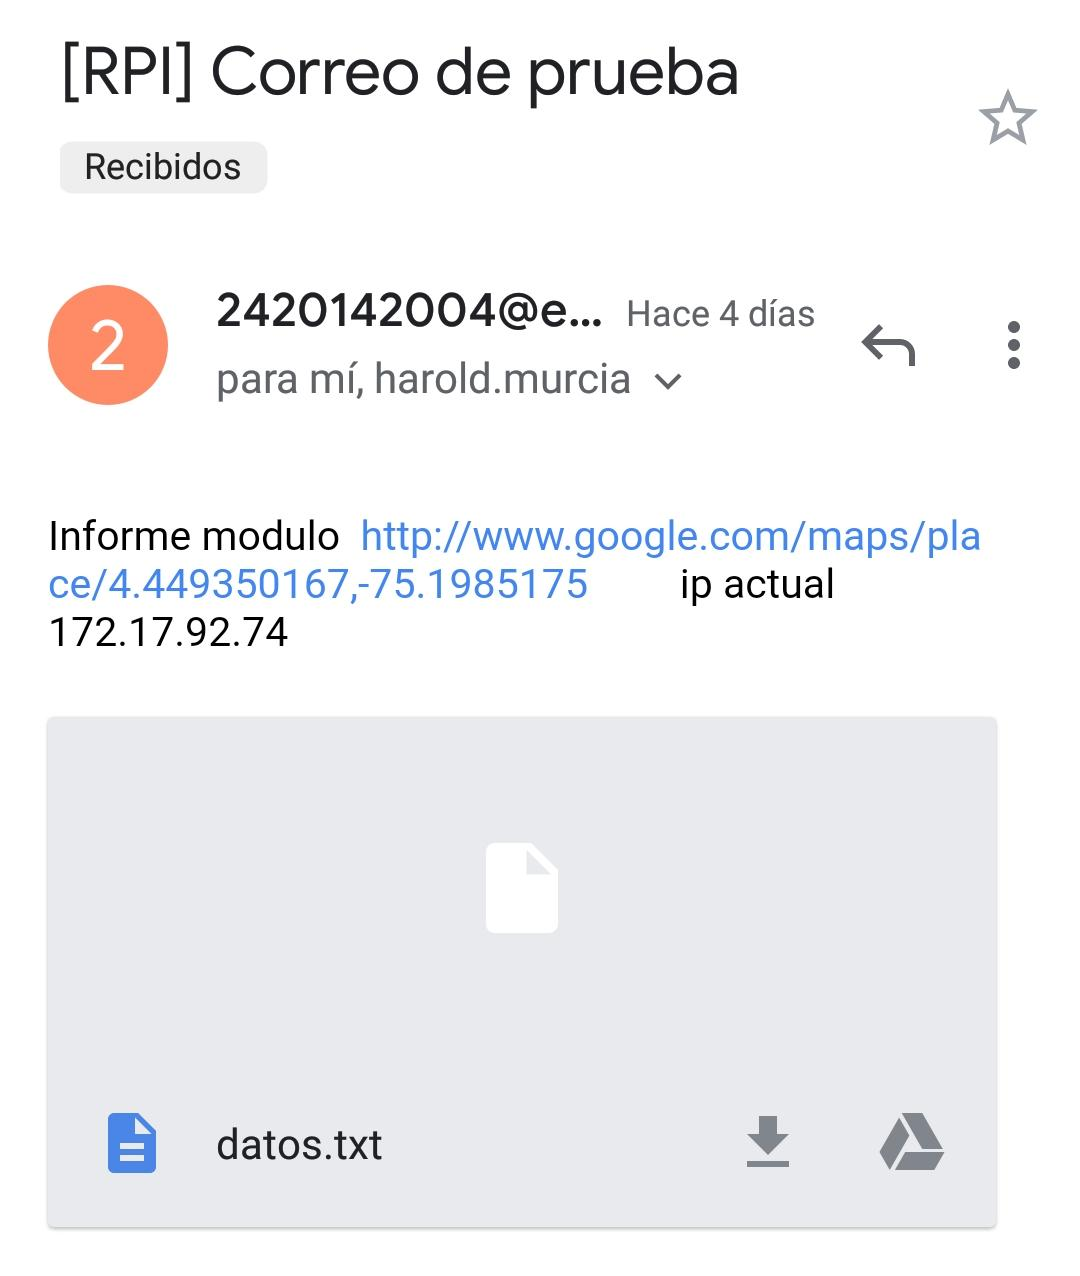
\includegraphics[width=0.3\textwidth]{gmail.jpeg}
\\
\caption{Fig[5] E-mail Sent}
\end{center}



\begin{center}
\section{CONCLUSIONS}
\end{center}

• The sending of the sensors reading to the ThingSpeak web platform has a waiting time of 20 seconds, because the platform does not generate any data collection before 15 seconds of sending.

• The email sending function was correctly functioning every 12 Hours with information on the behavior of each sensor during that time, the location of the station and the IP address from where it is being controlled.

• During the implementation of the GPS module, we had problems when initializing it, this because in most cases it did not detect the satellite, since the device is designed for free spaces, because during the test periods we worked in mostly closed spaces, we installed the GPS libraries again and we looked for a free space for a few seconds to continue with the tests.

• The air quality and rain sensors, presented complications at the time of their readings, this due to the transfer of data from the Arduino to the Raspi, since the implementation code for this function had syntax flaws, which we solved through installation of some libraries and hierarchy spaces within it.

• The implementation of the Internet of things IOT was achieved, which allowed us to visualize in real time the behavior of all our variables and their sending through Gmail.

• At the time of generating an independent source of energy for the system, we encountered the problem that some software functions demanded a lot of current consumption which did not allow it to last more than 20 seconds in operation, or that the battery was discharged in A very short time. To solve this problem we add to our source code in each WHILE function, a Sleep of 0.5 seconds.

\begin{center}
\section{REFERENCE}
\end{center}


[1] Smartic Research Seedbed. (2015) Design and implementation of a prototype low-cost remote weather station using the internet of things approach. Recovered from: http://repository.unipiloto.edu.co
/bitstream/handle/20.500.12277/1008
/00002625.pdf?sequence=1

[2] Rojas, F. (2017). Construction of a low-cost weather station for climate monitoring, using 3D printing technology (Undergraduate Thesis). Major University of San Andrés, La Paz, Bolivia.

[3] Morkerker, L. (2019). Complete Raspberry Pi Weather Station [Blog]. Recovered from: https://www.instructables.com/id/C
omplete-Raspberry-Pi-Weather-Station /

[4] Ssja, J. (2019). Weather station [Blog]. Recovered from: https://www.instructables.com/id/Weather-Station-7 /

[5] Dr. Rafael Belloso Private University (2016, January1). Use of the low-cost mini-computer “raspberry pi” in Meteorological stations. Recovered from: https://www.redalyc.org/pdf/784/784
45977004.pdf

\end{multicols}
\\\\
\begin{center}
\textbf{ANNEXES}
\end{center}
\begin{center}
\text{ANNEXED.1 Weather Station}
\\
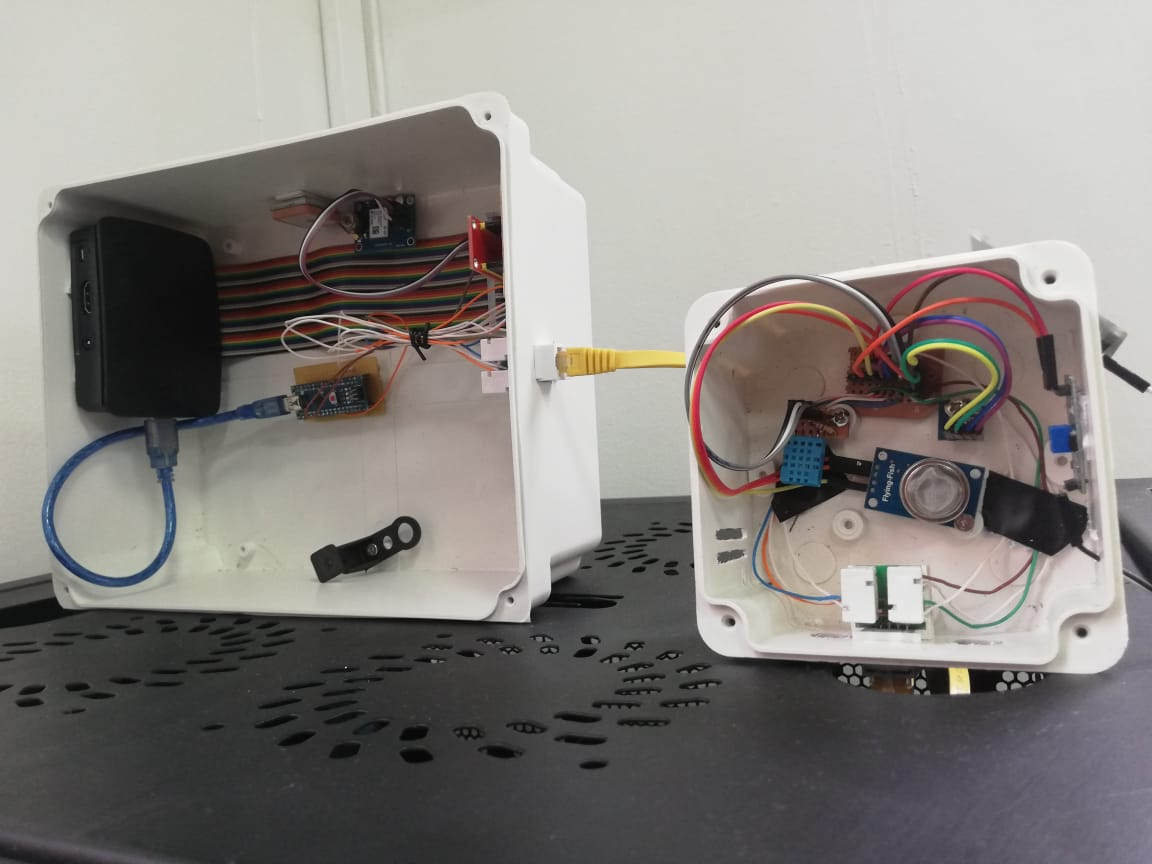
\includegraphics[width=0.4\textwidth]{ANEXO1.jpeg}
\end{center}
\\
\begin{center}
\text{ANNEXED.2 Thingspeak data}
\\
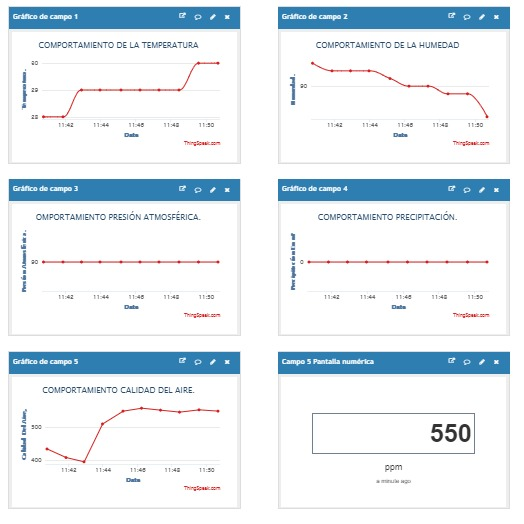
\includegraphics[width=0.4\textwidth]{grafico.jpg}
\end{center}
\\
\begin{center}
\text{ANNEXED.3 Data in .txt file}
\\
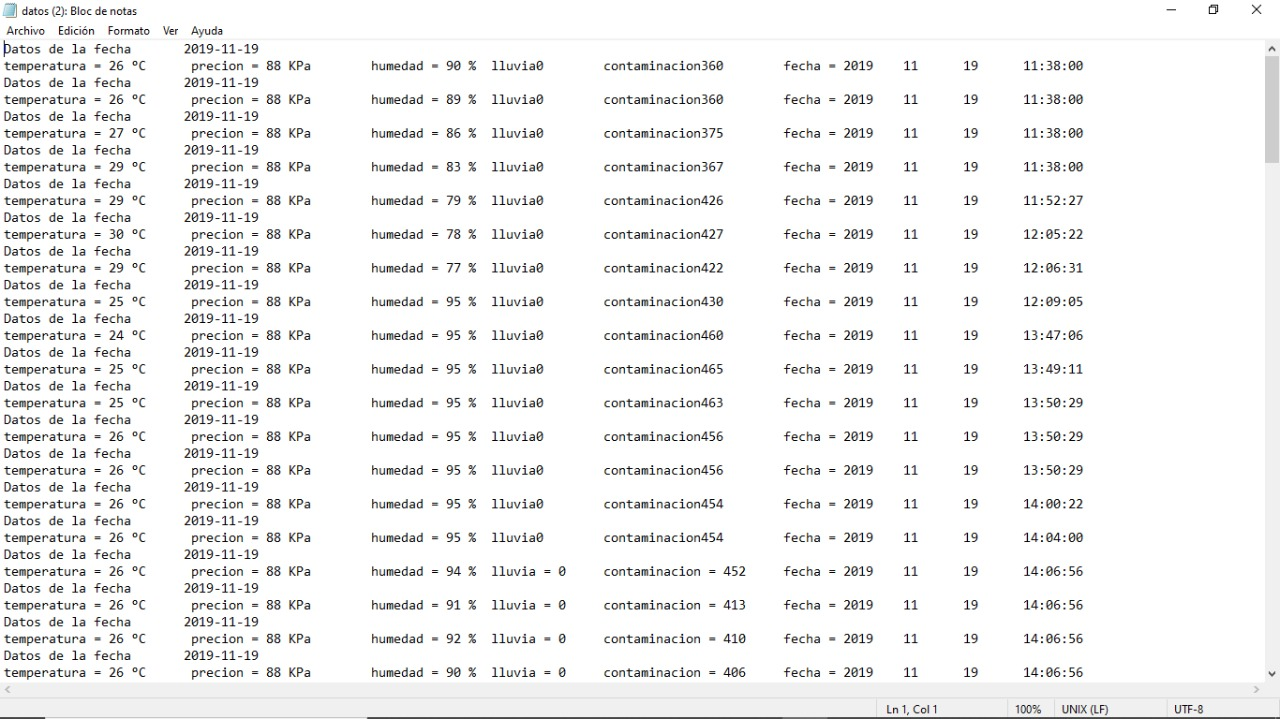
\includegraphics[width=0.9\textwidth]{diagrama.jpeg}
\end{center}
\end{document}



